Since gyrotrons are ECMs, the gyro-devices are classified according to their functionality and dispersion diagrams, that are designs based on a particular concept is the wave-particle interaction. Dispersion diagrams, also called w-kz plots or Brillouin diagrams, show the region of cyclotron interaction (maximum gain of the instability) between an electromagnetic mode and a fast electron cyclotron mode (fundamental or harmonic) as an intersection of the waveguide mode dispersion curve (hyperbola): $ w2 = k z^2 c^2 + k'^2 c^2 $

\section{Gyro-oscillators}
Gyro-oscillators are capable of providing high power in pulse mode or low power in CW (Continuous Wave) modes.  These gyrotrons are now being used in short and long pulse Megawatt-class gyrotrons.
\subsection{Gyro-monotron}
Gyro-monotrons are generally referred as gyrotrons. These devices are a type of ECR (Electron Cyclotron Maser) that underwent major development.  In 1964, IAP Nizhny Novgorod built and operated the first gyrotron in TE101 mode producing 6W power in CW mode. The device's output power increased when the originally used electron gun was replaced by Magnetron Injection Gun in tapered, open-ended waveguide cavities that maximize efficiency by tailoring the electric field distribution in the resonator. These devices are operated at resonant frequencies (see figure \ref{fig:gmd} ) Some times, the gyrotron can be operated at higher harmonics with lower fundamental frequencies and efficiencies.

\subsection{Gyro-BWO}
Gyro-BWO(Back Ward Oscillators) are similar to gyro-monotrons except for the wave interaction where the electron beam and/or magnetic field is adjusted so that the straight fast-wave beam line crosses the negative kz-branch of the waveguide mode (see figure \ref{fig:gbd} ) creating instability by because of a backward-wave (internal feedback). These devices are used to generate moderately high power, but work at relatively lower frequencies and efiiciencies compared to the standard gyrotron.\cite{ref:bwo}

\begin{figure}[H]
\centering
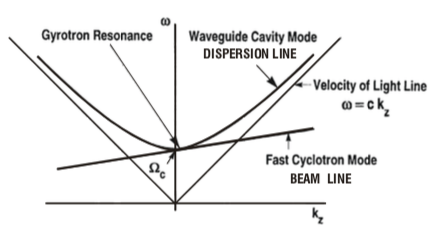
\includegraphics[scale=0.8]{images/gyro_mono_dispersion}
\label{ fig:gmd }
\caption{Dispersion diagram of Gyro-monotron}
\end{figure}
\begin{figure}
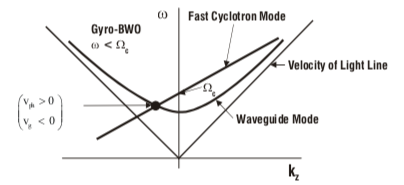
\includegraphics{images/gyro_bwo_dispersion}
\label{ fig:gbd }
\caption{Dispersion diagram of Gyro-BWO.}
\end{figure}



\subsection{Performance}
The following tables short-pulsed gyrotron and relativistic pulse gyro-BWOs (tables \ref{tab:spgm} and \ref{tab:spgb} ).

\begin{table}[H]
	\begin{tabular}{c|c|c|c|c}
	Institution & Frequency (GHz) & Cavity Mode & Power (MW) & Efficiency (\%) \\
	\hline
	CPI/MIT/GA & 110 & TE22,6 cylindrical & 1.5 & 48 (SDC)\\
	FZK/EFDA & 165 &TE31,12 coaxial & 2.2 & 48 (SDC)\\
	GYCOM/IAP & 170 & TE28,12 cylindrical &1.44 & 41 (SDC)\\
	TED/EFDA & 170 & TE34,19 coaxial & 1.8 & 28\\
	Toshiba/JAEA & 170 & TE31,12 cylindrical & 1.56 & 27
	\end{tabular}
	\caption{Short-Pulse 1.5–2 MW Gyro-monotrons\cite{ref:soa} }
	\label{tab:spgm}
\end{table}

\begin{table}[H]
	\begin{tabular}{c|c|c|c|c}	
	Institution & Frequency (GHz) & Cavity Mode & Power (kW) & Efficiency (\%) \\
	\hline
	IAP, N. Novgorod & 24.7 & TE1,1 & 7 & 7\\
	UNIV. Hsinchu & 33.5 & TE1,1 & 40 & 15
	\end{tabular}
	\caption{Relativistic Short-Pulse Gyro-BWO\cite{ref:soa} }
	\label{tab:spgb}
\end{table}

The above metrics\cite{ref:soa} indicate that:
\begin{enumerate}
\item The standard gyrotron/gyro-monotron devices are capable of operating at very high frequencies (100+Ghz) and capable of giving an output power of 1-2 MW.
\item The gyro-BWO operate at relatively low frequency and output low power.
\item

Each of the gyro-oscillators have clear applications according to the requirements, but most applications use the standard gyrotron oscillators to exploit the property of generating high power.
\end{enumerate}


\section{Gyro-Amplifiers}
The devices that come under gyro-amplifiers are :
\begin{enumerate}
\item  Gyro-klystron
\item  Gyro-twystron
\item Gyro-TWT
\end{enumerate}

Gyro-amplifiers are being developed and deployed to fields where there's a need for coherence and instantaneous bandwidth. Gyro-amplifiers are huge in terms of weight and volume than state-of-the-art coupled- cavity TWT, but provide significantly higher power than the TWTs. The wide variety of radar applications for which gyro-amplifiers are now being considered which wasn't the case before due to the absence of powerful amplifiers at the required frequencies. The bandwidth requirement of the application determines the tube type:

\begin{enumerate}
\item Gyro-klystron for less than 1\% bandwidth
\item Gyro-twystron for 1\% to 2\% bandwidth
\item Gyro-TWT for bandwidths greater than 2\%
\end{enumerate}

\subsection{Gyro-Klystrons}
Conceptually, gyro-klystrons are gyrotron oscillators with an additional input cavity added to the structure ( see figure \ref{fig:gky} ). The operation of a gyro-klystron is similar to a conventional klystron except that electron bunching (gyro) occurs in the azimuthal than in axial direction. In a gyro-klystron,  the input signal is fed into input cavity, the new addition to the gyro-oscillator where the cyclotron bunching process is initiated. Then, the beam is passes through the tube as bunches form. As the beam passes through a second cavity, the amplified signal may be removed or the bunching process may be enhanced and the signal removed in a subsequent cavity.

\begin{figure}[H]
\centering
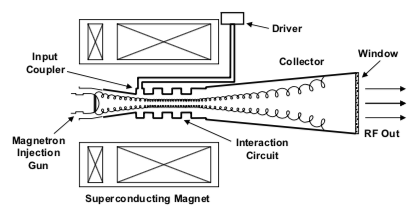
\includegraphics[scale=0.8]{images/gyro_klystron}
\label{ fig:gky }
\caption{Gyro-klystron}
\end{figure}

\subsection{Gyro-Twystron}
The gyro-twystron, is very similar to the conventional twystron, which is a hybrid device with a moderate bandwidth. The structure is derived from the gyro-klystron by using the gyro-klystron's interaction in the cavities near the RF input, but by replacing the output cavity with a slightly tapered waveguide section as in the gyro-TWT. The output section is excited by the electron beam, which is bunched by the interaction in the klystron section. This structure of the gyro-twystron doesn't suffer with the problem of having a breakdown at high-power levels because the radio frequency power density in the output waveguide is smaller than in the gyro-klystron output cavity.

\subsection{Gyro-TWT}\cite{ref:pkmm}
Of all the gyro-amplifiers, the gyro-TWT has gathered the most interest and research development. In millimetre-wave radars, the gyro-TWT is a proper fit as the transmitter power amplifier. Gyro-TWTs are capable of a much broader bandwidth than gyro-klystrons.
In gyro-TWTs, a nonresonant RF structure is used to produce a traveling wave interaction unlike in other gyro-devices, a spiraling electron beam immersed in an axial magnetic field is used. Traveling waves are launched into the interaction space by an input coupler. As the spiraling electron beam moves through the interaction space along with the electromagnetic wave, it loses energy to the electromagnetic field i.e is transferred into the electromagnetic fields, creating RF amplification. In a usual operation, the device is operated near the cutoff frequency of the interaction waveguide, where the transverse component of electron motion that interacts with the electromagnetic wave (in the same direction) .

Most of the interaction space exhibits a moderate amount of electromagnetic loss per unit length to ensure stability of the device. This distributed loading approach has been shown to have superior stability characteristics. Finally, the downstream part of the interaction space is completed with a short, unloaded cylindrical tunnel in which the final, highest powered portion of the amplification takes place.

\subsection{Performace}
The following tables comprises data of relativistic short-pulsed gyro-klystron,  short-pulse gyro-twystrons and short-pulse gyro-TWTs (tables \ref{tab:spgk}, \ref{tab:spgt}, \ref{tab:spgtw} ).

\begin{table}[H]
	\resizebox{\columnwidth}{!}{
	\begin{tabular}{c|c|c|c|c|c|c}	
	Institution & Frequency (GHz) & Cavity Mode & No. of Cavities & Power (MW) & Efficiency (\%) & Bandwidth(\%) \\
	\hline
	UNIV. Maryland & 8.57 & TE0,1 & 3 & 75 & 32 & 0.2\\
	IAP, Nizhny Novgorod & 30 & TE5,3 & 2 & 5 & 25 & 0.14
	\end{tabular}}
	\caption{Relativistic Short-Pulse Gyro-Klystrons\cite{ref:soa} }
	\label{tab:spgk}
\end{table}

\begin{table}[H]
	\resizebox{\columnwidth}{!}{
	\begin{tabular}{c|c|c|c|c|c|c}
	Institution & Frequency (GHz) & Cavity Mode & No. of Cavities & Power (MW) & Efficiency (\%) & Bandwidth(\%) \\
	\hline
	UNIV. Maryland & 9.87 & TE0,1 & 2 & 21.6 & 21 & 1-2\\
	UNIV. Maryland & 19.76 & TE0,1 & 2 & 12 & 11 & 1-2
	\end{tabular}}
	\caption{Relativistic Short-Pulse Gyro-Twystrons\cite{ref:soa} }
	\label{tab:spgt}
\end{table}

\begin{table}[H]
	\resizebox{\columnwidth}{!}{
	\begin{tabular}{c|c|c|c|c|c|c}
	Institution & Frequency (GHz) & Cavity Mode & No. of Cavities & Power (MW) & Efficiency (\%) & Bandwidth(\%) \\
	\hline
	IAP, Nizhny Novgorod & 79.4 & TE1,1 & & 1.1 & 29 & 2.1\\
	NRI, Washington D.C & 35 & TE1,1 & &20 & 11 & NA
	\end{tabular}}
	\caption{Relativistic Short-Pulse Gyro-TWTs\cite{ref:soa} }
	\label{tab:spgtw}
\end{table}

The above metrics\cite{ref:soa} indicate that as mentioned in the introduction of gyro-amplifiers, each of the devices has specific use cases based on the required bandwidth.
\begin{enumerate}
\item Gyro-klystrons are the most efficient gyro-amplifiers operating at releatively low frequencies and bandwidth.
\item Gyro-twystrons, compared to the other two amplifiers, operates at lower frequency with lower efficiency, only advantage being the operation bandwidth.
\item Gyro-TWTs are efficient devices capable of operating at higher frequencies and higher bandwidth.

Gyro-TWTs and gyro-klystrons are clear choices for applications requiring high output power like radars, where these devices are now being used.

\end{enumerate}
